\chapter{System Overview}
\label{ch:overview}

\section{Proposed solution}
Figure~\ref{fig:overview} shows the whole system. Clients, freelancers and arbiters use one web application in the browser. It sends every request to a REST API, which checks who the user is and what role they have before doing anything. Behind the API are three services:

\begin{itemize}
\item a private database that holds accounts, jobs, proposals, milestones and the history of each milestone;
\item a risk service that sends the payout wallet to the Python risk engine and stores the score, the reason and the action;
\item a chain service that deploys one escrow contract per job and sends every payment action to it.
\end{itemize}

Only the escrow contract runs on the blockchain. It stores the state of each milestone, the risk flag and its reason, and nothing about the users beyond their addresses. The money moves only when the contract's rules allow it, so the database is never the authority on payments: after every action the API reads the milestone back from the contract and copies its state.

\begin{sidewaysfigure}
\centering
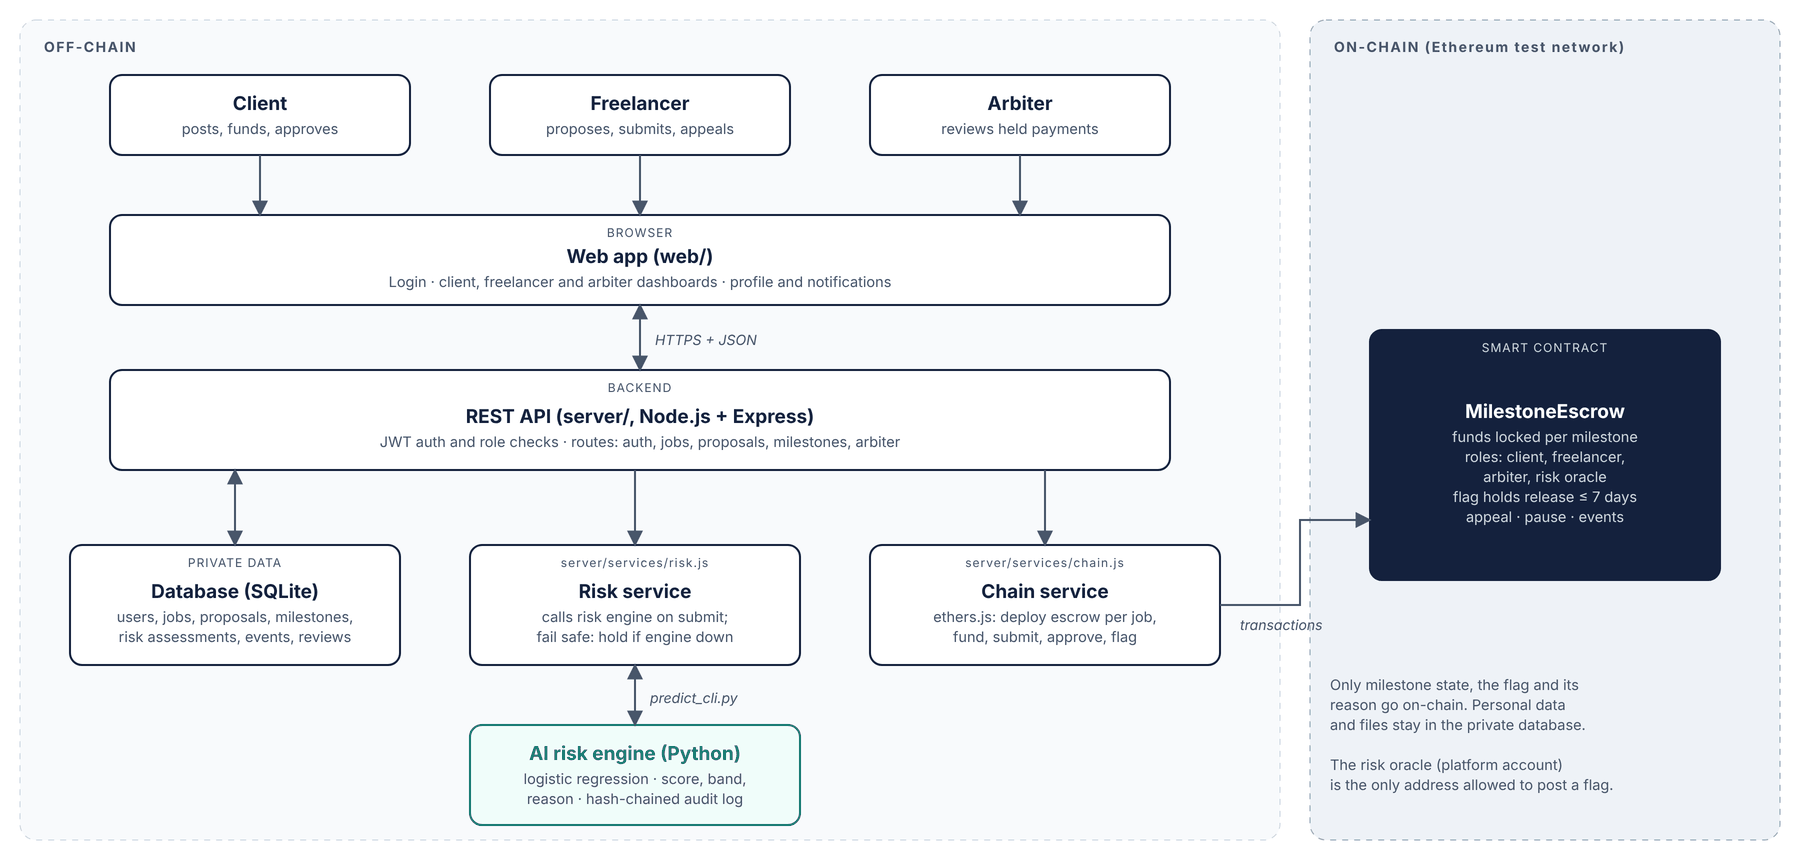
\includegraphics[width=\textheight]{figures/overview.png}
\caption{System overview. Everything on the left runs off-chain; the escrow contract on the right is the only on-chain part.}
\label{fig:overview}
\end{sidewaysfigure}

\section{Actors}
\begin{table}[htbp]
\centering
\small
\begin{tabularx}{\textwidth}{>{\raggedright\arraybackslash}p{3.2cm}L}
\hline
\textbf{Actor} & \textbf{What they do} \\ \hline
Client & Posts jobs, accepts a proposal, adds and funds milestones, approves or disputes submitted work. \\
Freelancer & Browses open jobs, sends proposals, submits work, appeals a risk flag. \\
Arbiter & Reviews flagged and disputed milestones, releases or refunds them, and can pause a job's contract in an emergency. \\
Risk engine (system) & Scores the payout wallet when work is submitted and, when the score is high, has the risk oracle post the flag and reason on-chain. \\
Smart contract (system) & Holds the funds and enforces who may release or refund them. \\ \hline
\end{tabularx}
\caption{Actors and their responsibilities.}
\label{tab:actors}
\end{table}

\section{Technology}
\begin{table}[htbp]
\centering
\small
\begin{tabularx}{\textwidth}{>{\raggedright\arraybackslash}p{3.2cm}L}
\hline
\textbf{Part} & \textbf{Technology} \\ \hline
Smart contract & Solidity 0.8.24, tested with Hardhat and ethers.js \\
Backend & Node.js, Express, JSON Web Tokens, scrypt password hashing \\
Database & SQLite, run through sql.js so it installs on any operating system without build tools \\
Risk engine & Python 3, pandas, scikit-learn (logistic regression~\cite{hosmer,sklearn}) \\
Web application & HTML, CSS and JavaScript with no framework or build step \\
Blockchain (now) & Hardhat's local test chain with test ETH \\ \hline
\end{tabularx}
\caption{Technology used in each part of the system.}
\label{tab:tech}
\end{table}
